\documentclass[%
  a4paper,%
  11pt,% <10pt, 9pt>
  %style=screen,
  %sender=bottom,
  blue,% <orange, green, violet>
  %rgb, <cmyk>
  %mono,
  hyperref	% tubs color for hyperref
  ]{tubsartcl}
\usepackage[utf8]{inputenc}
\usepackage{hyperref}

\setlength{\parindent}{0cm}
 
% Titelseiten-Elemente
\title{TuringBrain IDE \LARGE 1.0}
\subtitle{User Guide}
\author{\small Vanessa Baier, Nils Breyer, Phillipp Neumann,\\ Sven Schuster, David Wille}
\logo{
\includegraphics{ips}}
\titleabstract{TuringBrain IDE -- User Guide}
\titlepicture{title}
% Rückseiten-Elemente
\address{
  Advisor: Matthias Hagner\\\\
  Technische Universität Braunschweig\\
  Institut für Programmierung und Reaktive Systeme\\
  Mühlenpfordtstr. 23\\
  38106 Braunschweig}
\backpageinfo{
}

\begin{document}

\maketitle[image,logo=right]%[<plain/image/imagetext>,<logo=left/right>]

\tableofcontents
\newpage
\section{Introduction}

TuringBrain IDE allows you to develop and debug your own TuringMachines in an easy to use WYSIWYG (what you see is what you get) environment. It also enables you to program and run Brainfuck code.

\subsection{Features}

\begin{itemize}
  \item Edit Turing Machines by graphically editing the state graph
  \item Create Turing Machines with multiple tapes
  \item Write Brainfuck programs within the integrated code editor
  \item Simulate your machines and programs using the integrated simulation
  \item Simulate on special LEGO-Tape (hardware needed), graphically animated on the screen or on the console
  \item Pause simulation, Debug step-by-step
  \item Live-highlighting of the current state and edge during the simulation
  \item Save machines as .tm (an XML-Format) respective .bf
  \item Copy \& Paste (just for transitions on edges), Undo \& Redo
  \item Export to Latex, SVG, and PNG
  \item and many more features...
\end{itemize}

\section{Getting started}

\subsection{Installation}
\label{sec:installation}
If you don't want to use the LEGO tapes, you only have to download the executable .jar file from our repository.
To use the LEGO tapes you have to do following steps:
\begin{enumerate}
	\item Download Version 0.8.5beta of LeJos from http://sourceforge.net/projects/lejos/files/lejos-NXJ/
	\item Download JGraph from http://www.jgraph.com/jgraph.html
	\item Unpack the archive to a folder where you have execute privileges
	\item Download eclipse an install it
	\item Checkout our project as a new project with the wizzard of eclipse
	\item Choose in the wizzard Libraries and add the variable for jgraph-home and nxj-home
	\item Finish the project wizzard and compile the PC components with the external tool
	%%Wahrscheinlich noch nicht ganz fertig%%
\end{enumerate}


\newpage

\subsection{Welcome page}
\label{sec:welcome-page}
If the installation was correct and you have started the application the one or the other way you will see the welcome page like in figure \ref{pic:welcome_page}. Now you can open a turing machine, create a new one or open an example that is listed below. \\
You can also do the same with a brainfuck program.
\begin{figure}[!htb]
\begin{center}
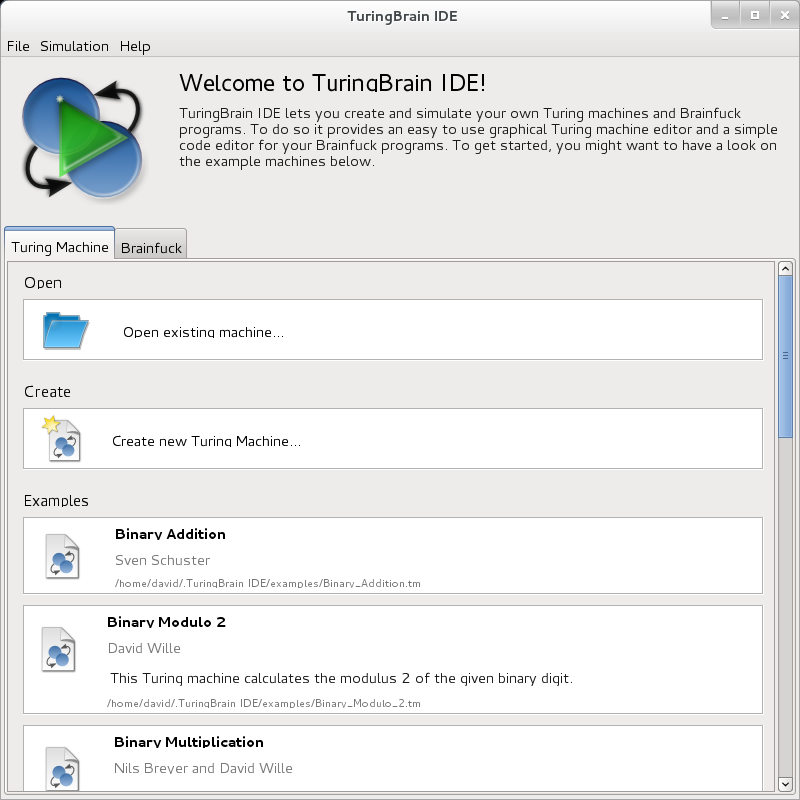
\includegraphics[scale=0.45]{graphics_gui/welcomescreen.png}
\end{center}
\caption{Welcome page}
\label{pic:welcome_page}
\end{figure}

\newpage

\section{Turing Machine editor}
If you open an example you will see a window like figure \ref{pic:turing_editor}, if you create a new turing machine you will have a blank page. On the left side you have the toolboxes in the white main part you can edit/create the turing machine.
\begin{figure}[!htb]
\begin{center}
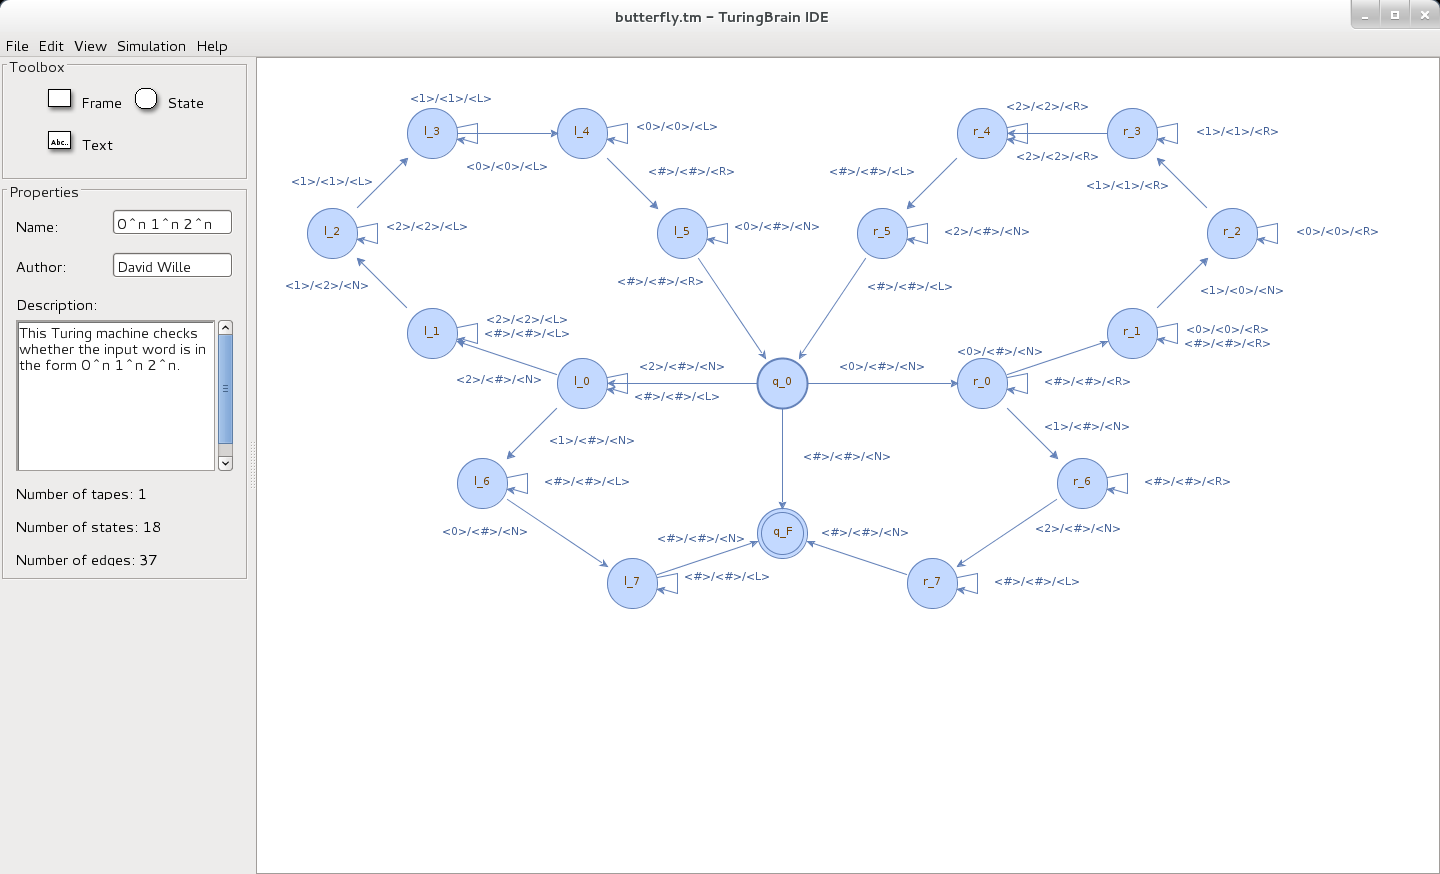
\includegraphics[scale=0.3]{graphics_gui/turing_editor.png}
\end{center}
\caption{Turing Machine editor}
\label{pic:turing_editor}
\end{figure}

\newpage

\subsection{Edit machine properties}
\label{sec:edit-mach-prop}
First of all you sould edit the turing machine properties.
\begin{figure}[!htb]
\begin{center}
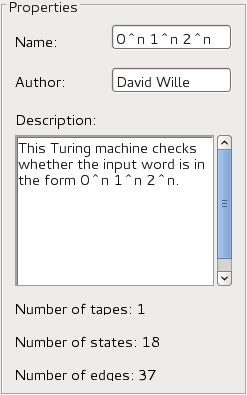
\includegraphics[scale=0.5]{graphics_gui/machine_properties.png}
\end{center}
\caption{Edit machine properties}
\label{pic:machine_properties}
\end{figure}

\newpage

\subsection{Toolbox}
\label{sec:toolbox}
With the toolbox you can drag an drop states, frame and text boxes on the main frame. In the main frame you have the possibility to change the size of text and frame boxes. 
\begin{figure}[!htb]
\begin{center}
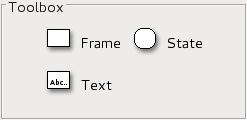
\includegraphics[scale=0.5]{graphics_gui/toolbox_turing.png}
\end{center}
\caption{Toolbox}
\label{pic:toolbox}
\end{figure}

\newpage

\subsection{Adding and changing states}
\label{sec:add-edit-states}
If you have created or selected a state you can change the properties of the selected state. You can specify a lable or if it is a start or final state. The start state will marked with a bold border and the final will marked with a second circle.
\begin{figure}[!htb]
\begin{center}
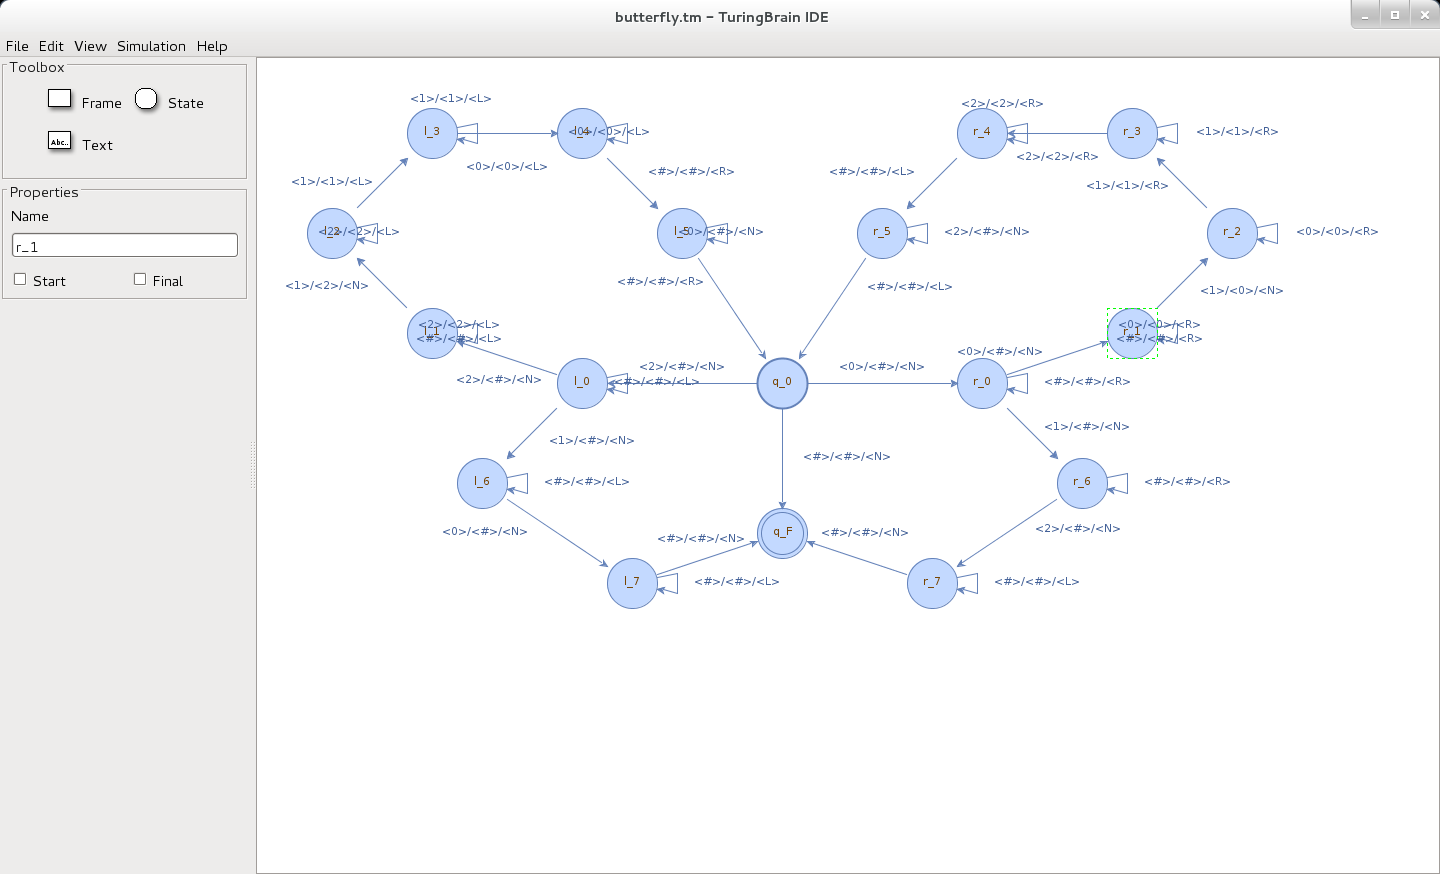
\includegraphics[scale=0.5]{graphics_gui/state_properties.png}
\end{center}
\caption{Adding and changing states}
\label{pic:state_properties}
\end{figure}

\newpage

\subsection{Adding and changing edges}
\label{sec:adding-chang-edges}
If you want to create an edge you have to move the mouse pointer in the center of a state the state will highlighted with a bold green square. Then you have to hold the left mouse key and drop the arrow on the state where the edge shall end. \\
If you have selected an edge you can add remove or edit trastions. If you want to edit a transition you have to double click an the trasition.
\begin{figure}[!htb]
\begin{center}
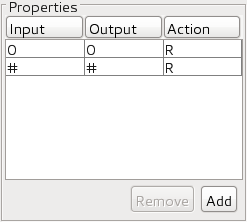
\includegraphics[scale=0.5]{graphics_gui/edge_properties.png}
\end{center}
\caption{Adding and changing edges}
\label{pic:edge_properties}
\end{figure}

\newpage

\subsection{Edit transitions}
\label{sec:edit-transitions}
If you double clicked a transtion or added a new, you can edit it. Allowed Input and output characters are \#, 0, 1, 2 and *, where * is a wildcard. Allowed actions are L (left), R (right) an N (nothing). With ok you save the transition.
\begin{figure}[!htb]
\begin{center}
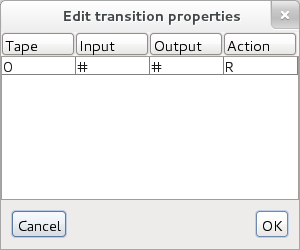
\includegraphics[scale=0.5]{graphics_gui/edit_transitions.png}
\end{center}
\caption{Edit transitions}
\label{pic:edit_transitions}
\end{figure}

\newpage

\subsection{Via points}
\label{sec:via-points}
In the Edit menu you can add a via point if you have selected an edge.
\subsection{Frames and textboxes}
\label{sec:frames-textboxes}

\begin{figure}[!htb]
\begin{center}
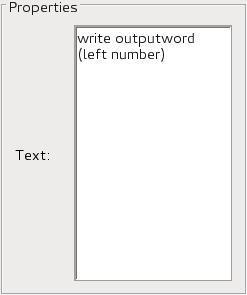
\includegraphics[scale=0.5]{graphics_gui/text_properties.png}
\end{center}
\caption{Textbox properties}
\label{pic:text_properties}
\end{figure}

\newpage

\subsection{Export}
\label{sec:export}

\newpage

\section{Brainfuck editor}

\begin{figure}[!htb]
\begin{center}
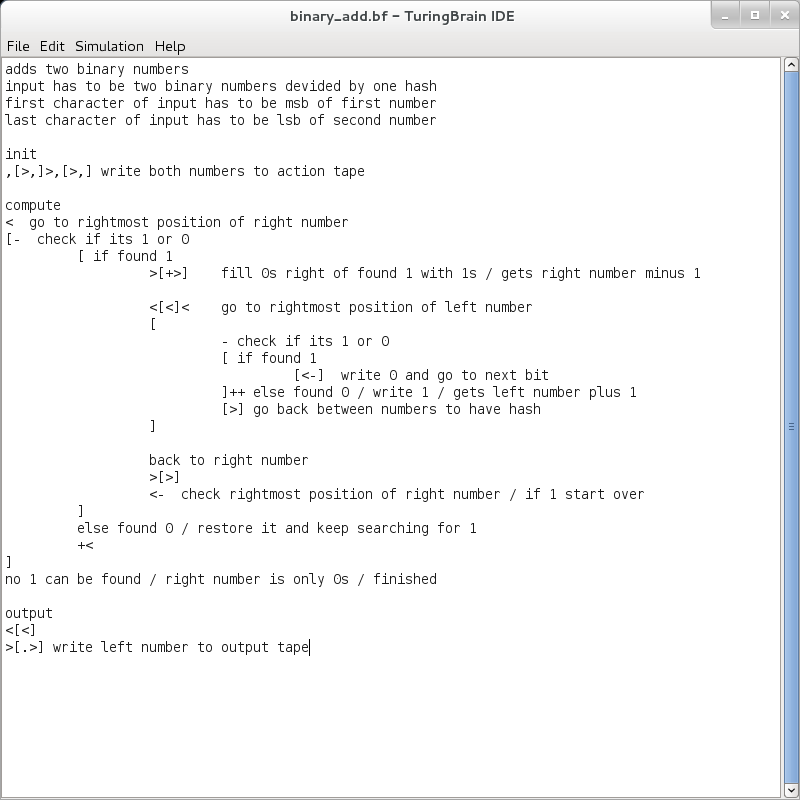
\includegraphics[scale=0.5]{graphics_gui/brainfuck_editor.png}
\end{center}
\caption{Brainfuck editor}
\label{pic:brainfuck_editor}
\end{figure}

\newpage

\section{Run window}

\begin{figure}[!htb]
\begin{center}
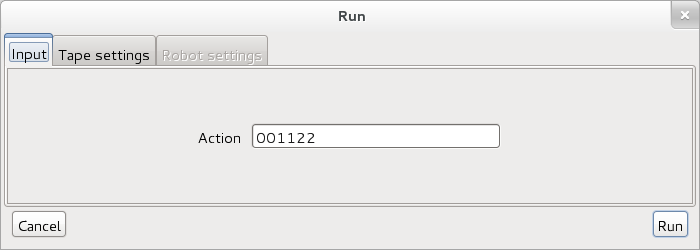
\includegraphics[scale=0.5]{graphics_gui/run_window_input.png}
\end{center}
\caption{Run window -- Input}
\label{pic:run_window_input}
\end{figure}

\newpage

\begin{figure}[!htb]
\begin{center}
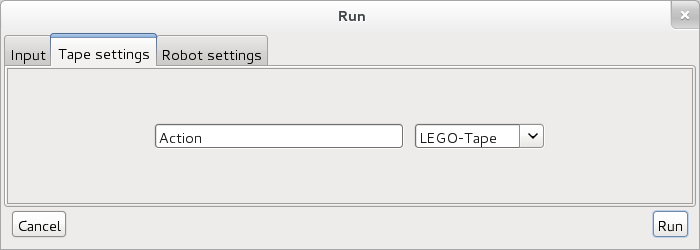
\includegraphics[scale=0.5]{graphics_gui/run_window_tape_settings.png}
\end{center}
\caption{Run window -- Tape settings}
\label{pic:run_window_tape_settings}
\end{figure}

\newpage

\begin{figure}[!htb]
\begin{center}
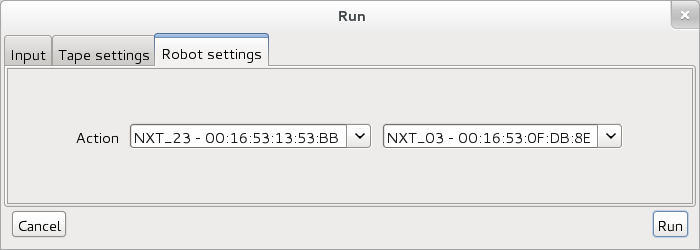
\includegraphics[scale=0.5]{graphics_gui/run_window_robot_settings.png}
\end{center}
\caption{Run window -- Robot settings}
\label{pic:run_window_robot_settings}
\end{figure}

\newpage

\section{Simulation}

\subsection{Organize robots}

\begin{figure}[!htb]
\begin{center}
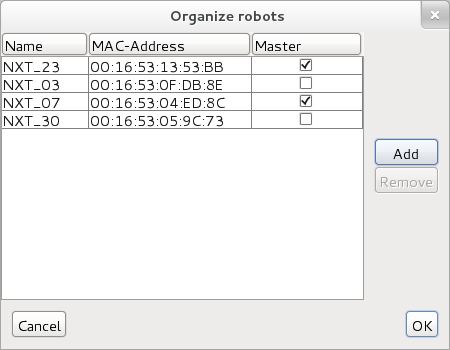
\includegraphics[scale=0.45]{graphics_gui/organize_robots.png}
\end{center}
\caption{Organize robots}
\label{pic:organize_robots}
\end{figure}

\newpage

\subsection{Presimulation window}

\begin{figure}[!htb]
\begin{center}
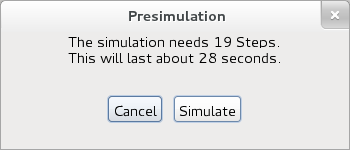
\includegraphics[scale=0.4]{graphics_gui/presimulation.png}
\end{center}
\caption{Presimulation window}
\label{pic:presimulation}
\end{figure}

\begin{figure}[!htb]
\begin{center}
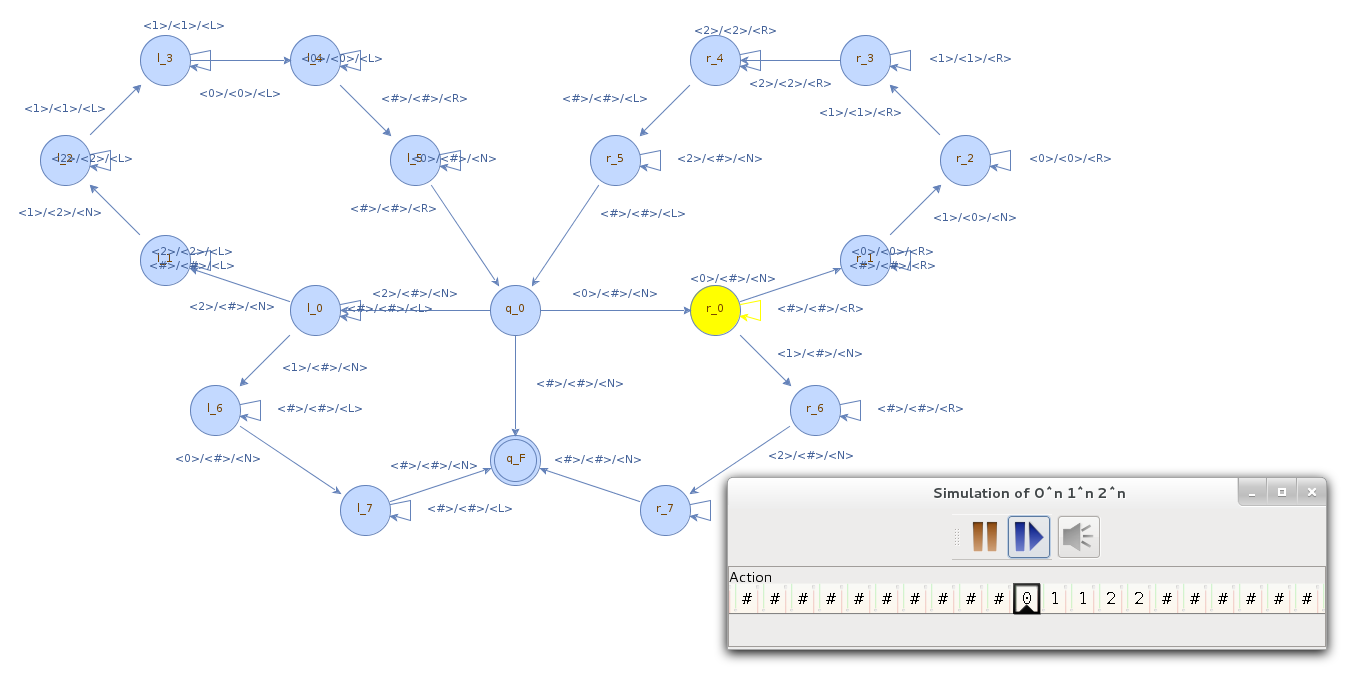
\includegraphics[scale=0.35]{graphics_gui/simulation_window.png}
\end{center}
\caption{Simulation window}
\label{pic:simulation_window}
\end{figure}

\newpage

\section{Hardware -- LEGO\textregistered\, tape}

This section describes the position of the components used in the machine. The following subsections and pictures are meant to extend the building instructions file created with the LEGO\textregistered\, Digital Designer.

\newpage

\subsection{Overview}

\begin{figure}[!htb]
\begin{center}
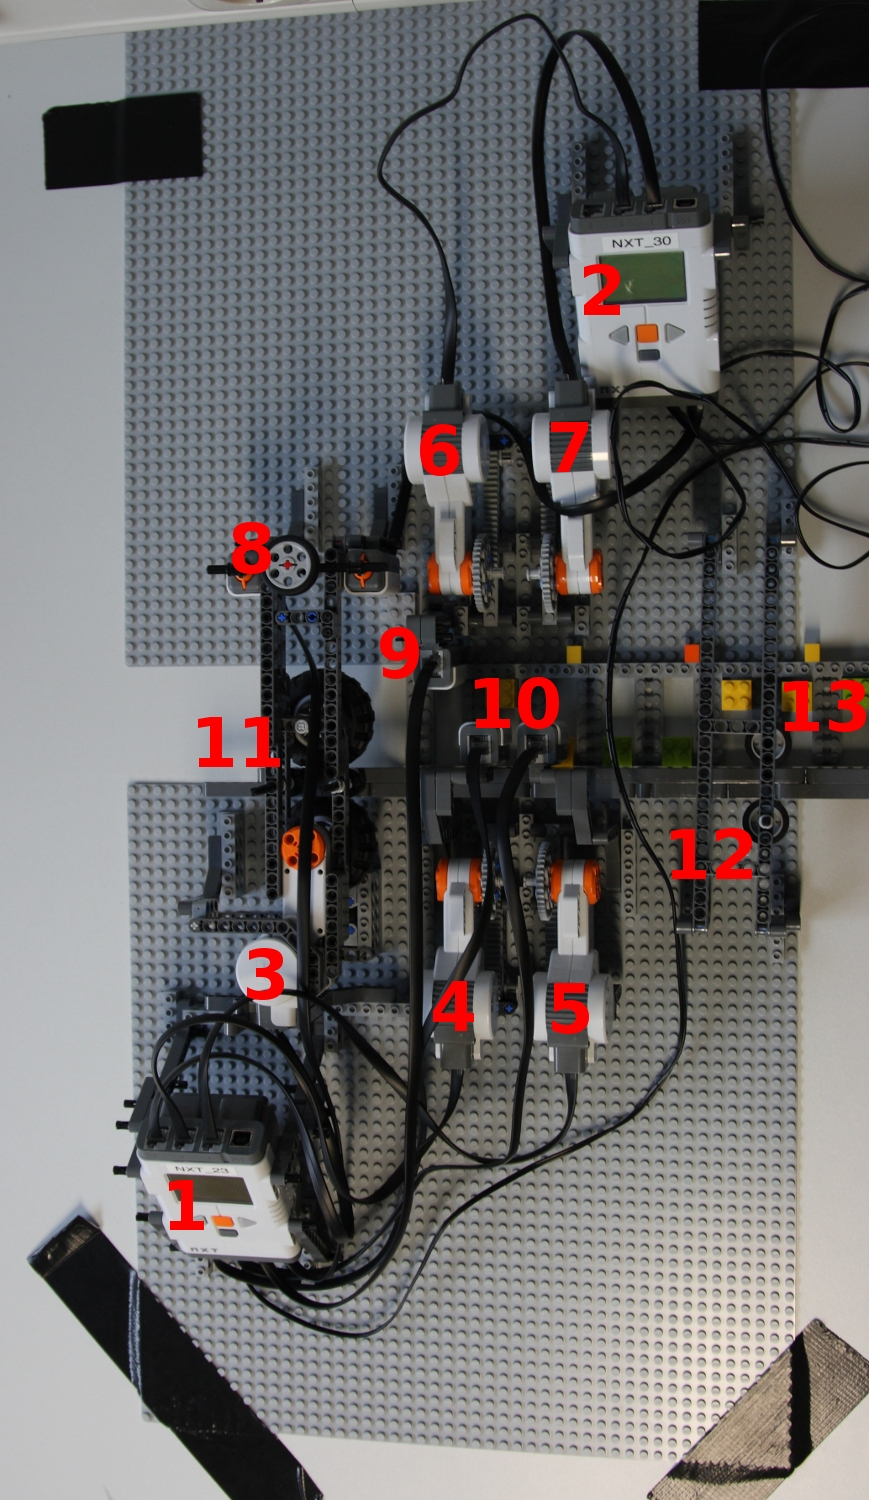
\includegraphics[scale=0.28]{graphics_lego/overview.jpg}
\end{center}
\caption{Overview of the LEGO\textregistered\, Turing Machine}
\label{pic:overview}
\end{figure}

\begin{center}
\begin{minipage}{6cm}
\begin{enumerate}
\item[1)] Master NXT module
\item[2)] Slave NXT module
\item[3)] Motor A master robot
\item[4)] Motor B master robot
\item[5)] Motor C master robot
\item[6)] Motor B slave robot
\item[7)] Emergency shutdown
\end{enumerate}
\end{minipage}
\begin{minipage}{8cm}
\vspace*{-1cm}
\begin{enumerate}
\item[8)] Motor C slave robot
\item[9)] Sensor to determine the tape position
\item[10)] Sensor to read the bits
\item[11)] Bridge with the machine's motor section
\item[12)] Bridge to support the tape
\item[13)] Tape
\end{enumerate}
\end{minipage}
\end{center}

\newpage

\subsection{The machine's motor section}

Figure \ref{pic:topview} shows a view of the machine's motor section to get a brief overview of it's position and the number 1 -- 4 represent the following pictures.

\begin{figure}[!htb]
\begin{center}
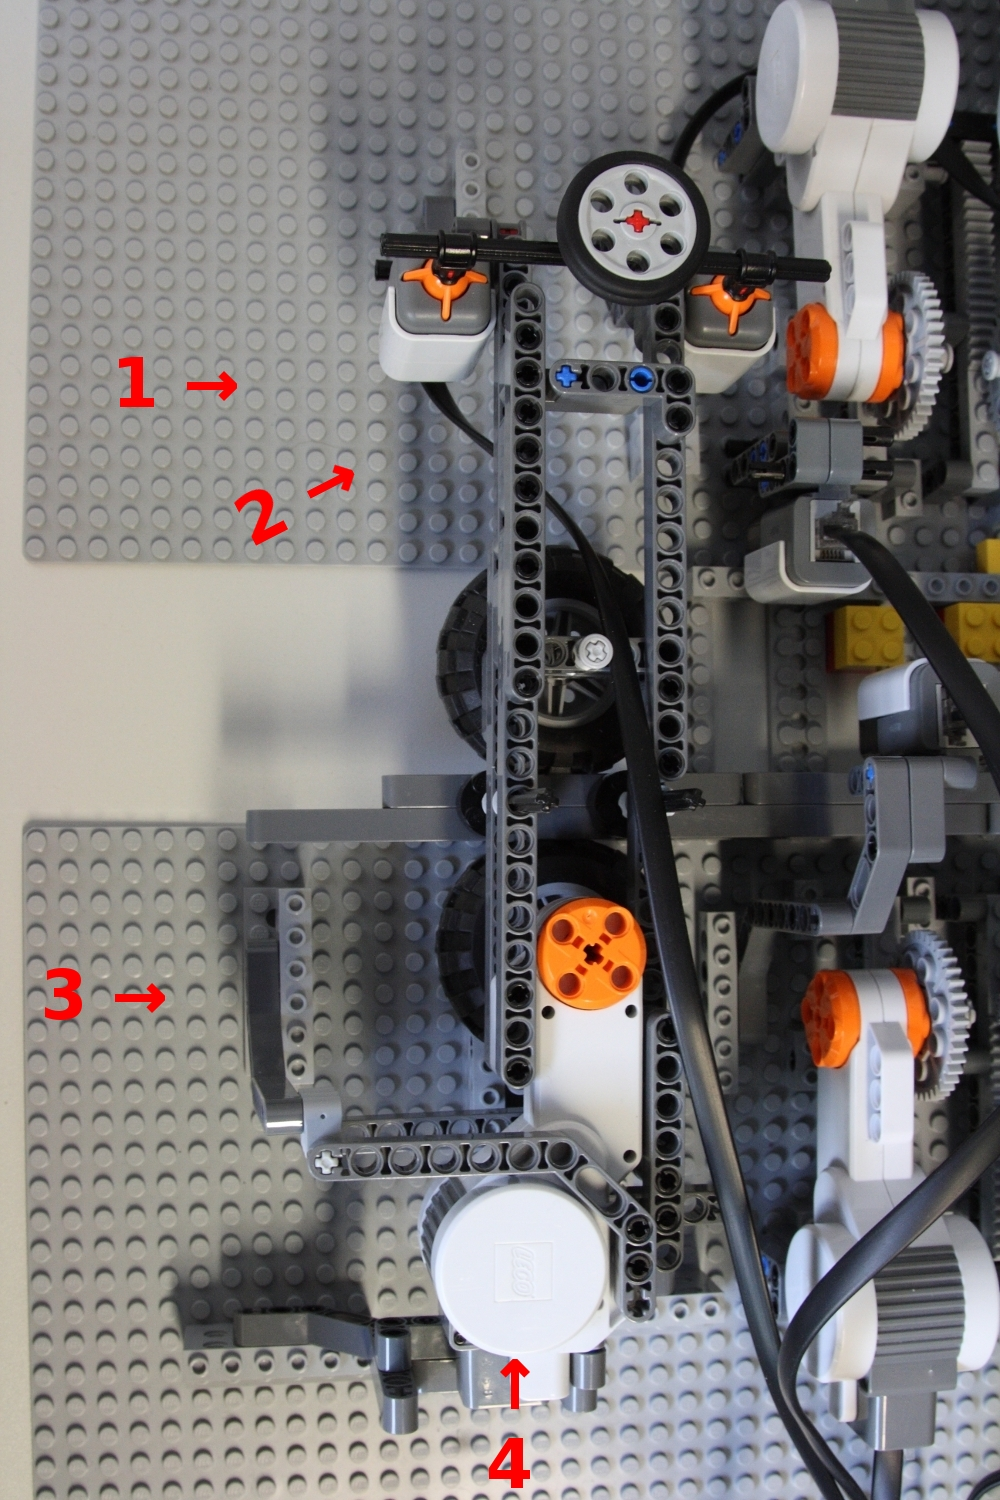
\includegraphics[scale=0.28]{graphics_lego/topview.jpg}
\end{center}
\caption{Overview of the motor section}
\label{pic:topview}
\end{figure}

\newpage

Figure \ref{pic:position1} shows how the upper left pier has to be placed in relation to the left edge of the upper plate.

\begin{figure}[!htb]
\begin{center}
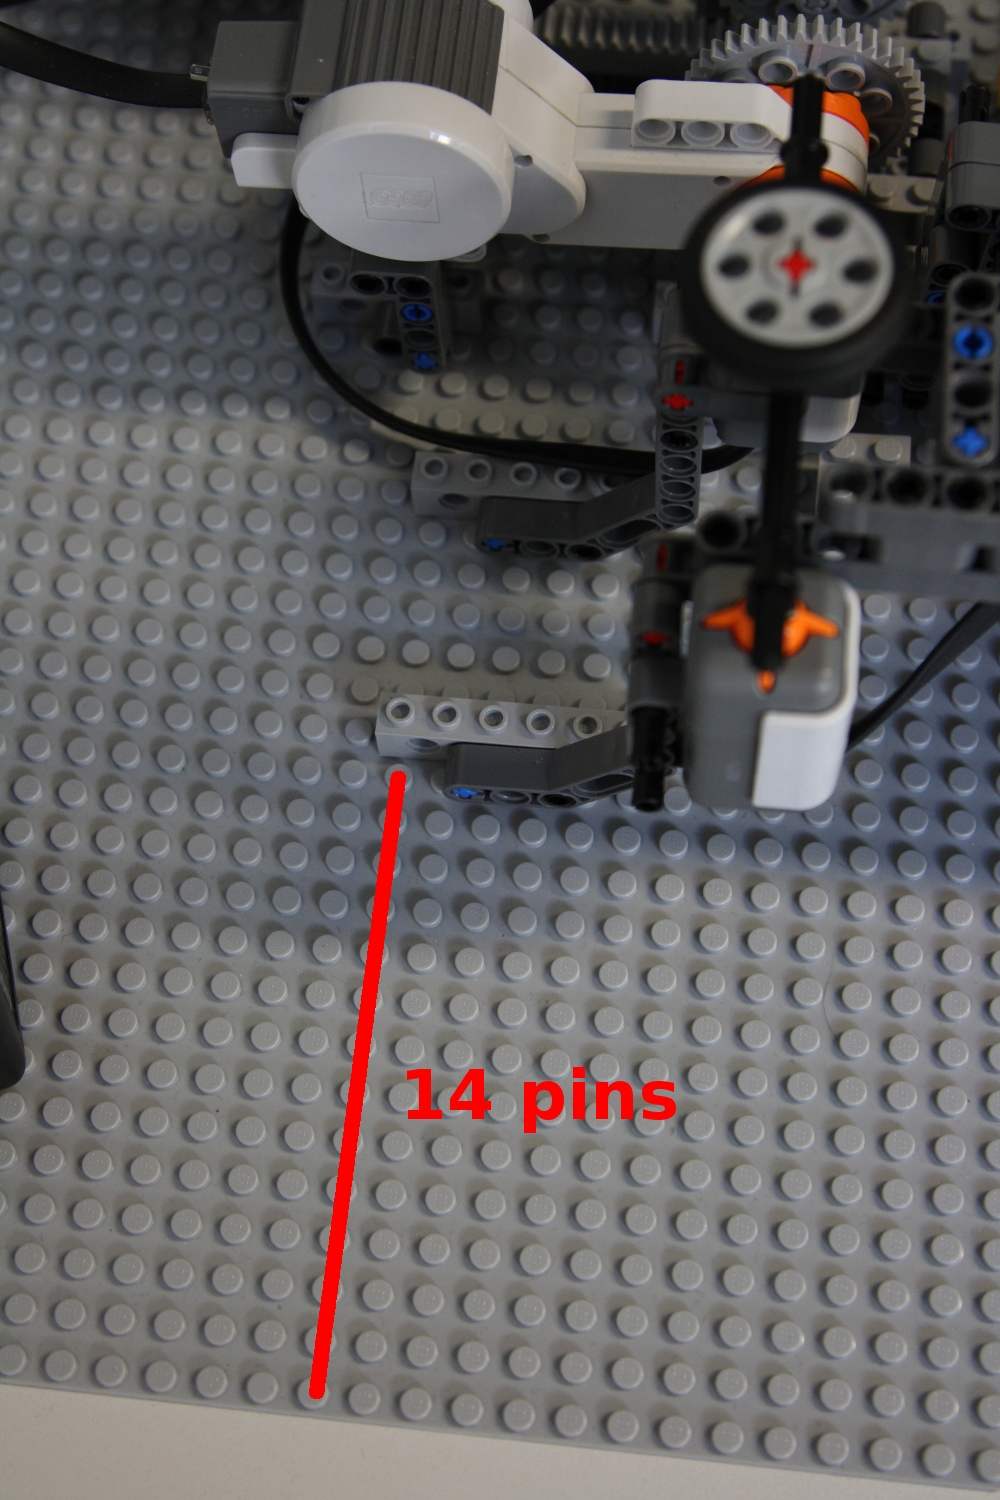
\includegraphics[scale=0.35]{graphics_lego/position1.jpg}
\end{center}
\caption{Image taken from position 1}
\label{pic:position1}
\end{figure}

\newpage

Figure \ref{pic:position2} shows how the upper left and right pier have to be placed in relation to the bottom edge of the upper plate.

\begin{figure}[!htb]
\begin{center}
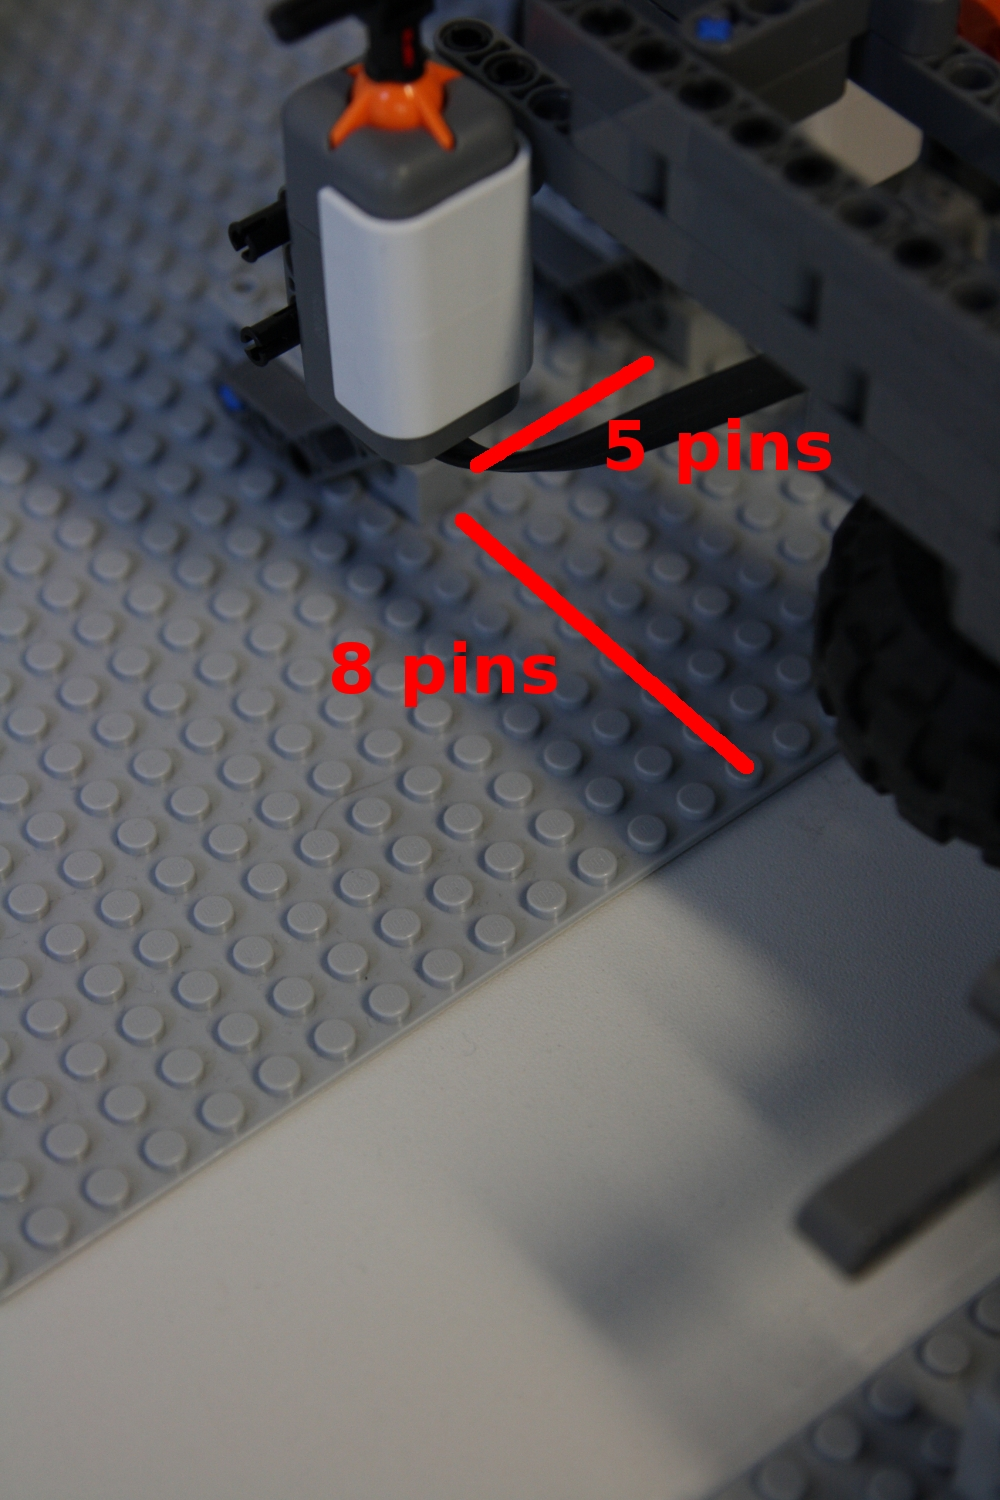
\includegraphics[scale=0.35]{graphics_lego/position2.jpg}
\end{center}
\caption{Image taken from position 2}
\label{pic:position2}
\end{figure}

\newpage

Figure \ref{pic:position3} shows how the lower left piers have to be placed in relation to the top and left edge of the lower plate.

\begin{figure}[!htb]
\begin{center}
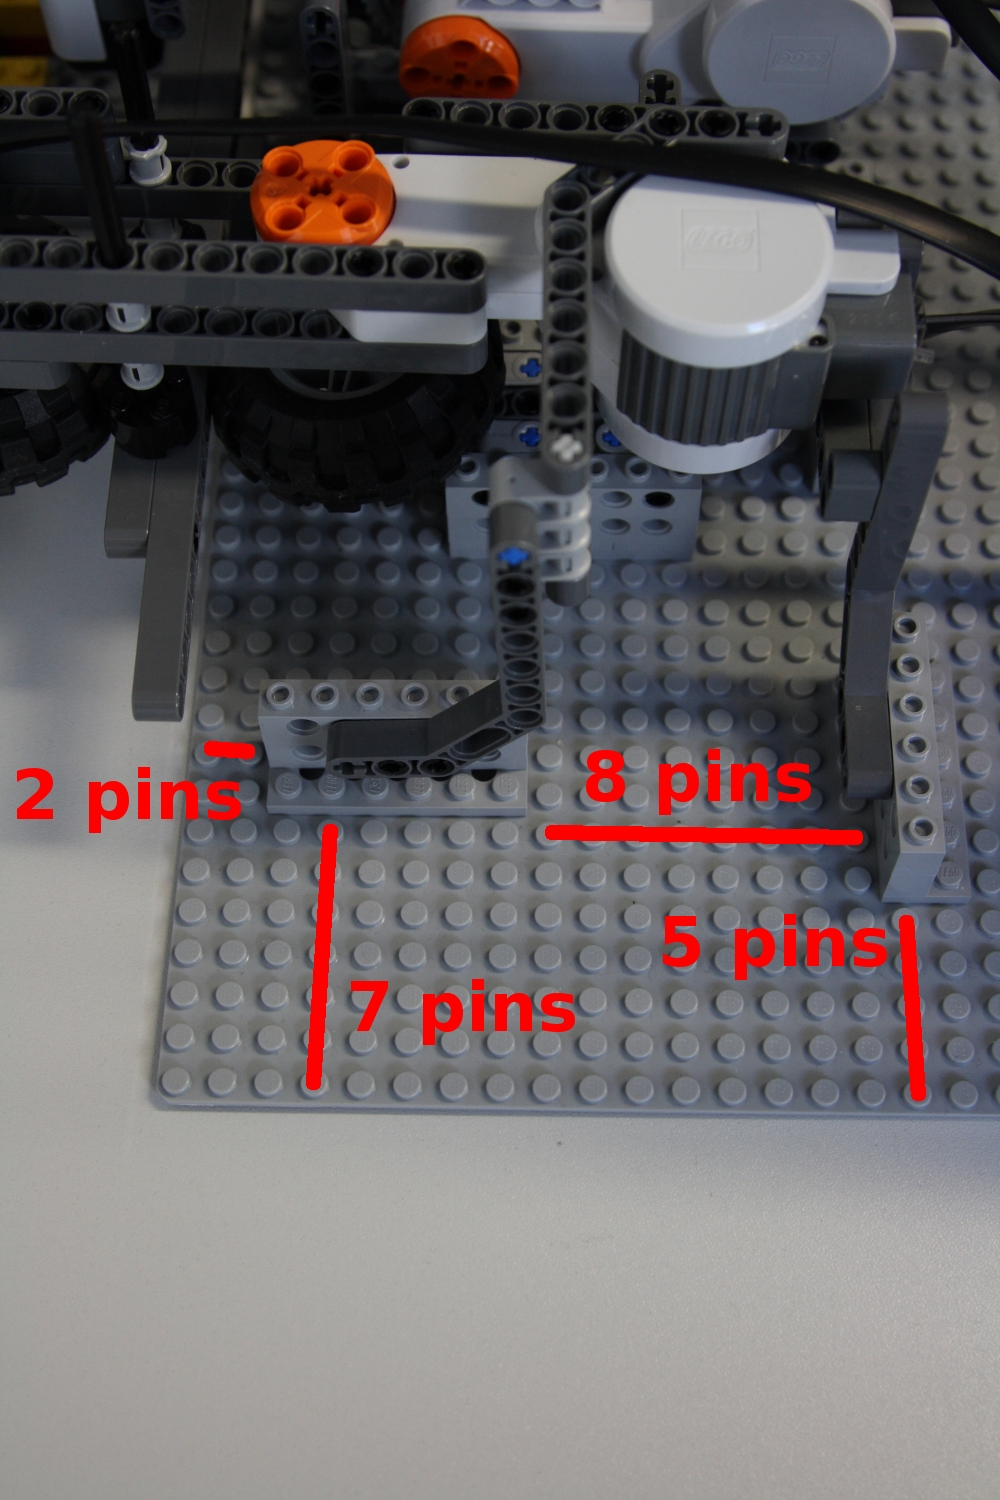
\includegraphics[scale=0.35]{graphics_lego/position3.jpg}
\end{center}
\caption{Image taken from position 3}
\label{pic:position3}
\end{figure}

\newpage

Figure \ref{pic:position4} shows how the lower right pier has to be placed in relation to the left pier and the support for the motor wheel.

\begin{figure}[!htb]
\begin{center}
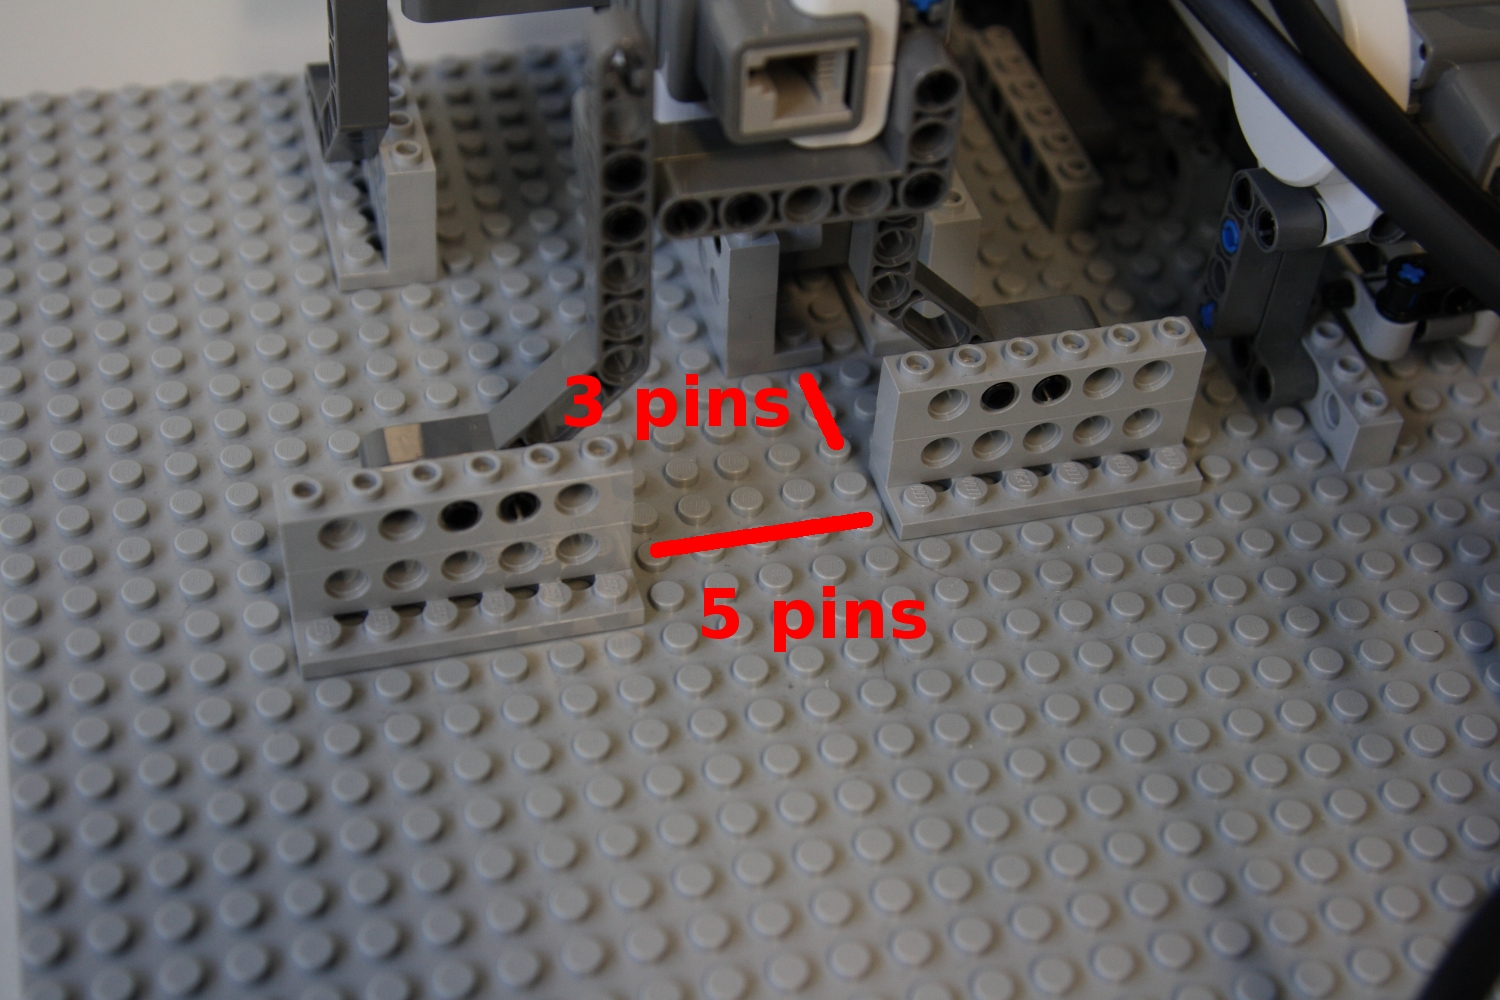
\includegraphics[scale=0.3]{graphics_lego/position4.jpg}
\end{center}
\caption{Image taken from position 4}
\label{pic:position4}
\end{figure}

\newpage

\subsection{The supporting bridge at the end of the tape}

Figure \ref{pic:bridge2} shows how the upper piers of the supporting bridge have to be placed in relation to the lower and right edge of the upper plate.

\begin{figure}[!htb]
\begin{center}
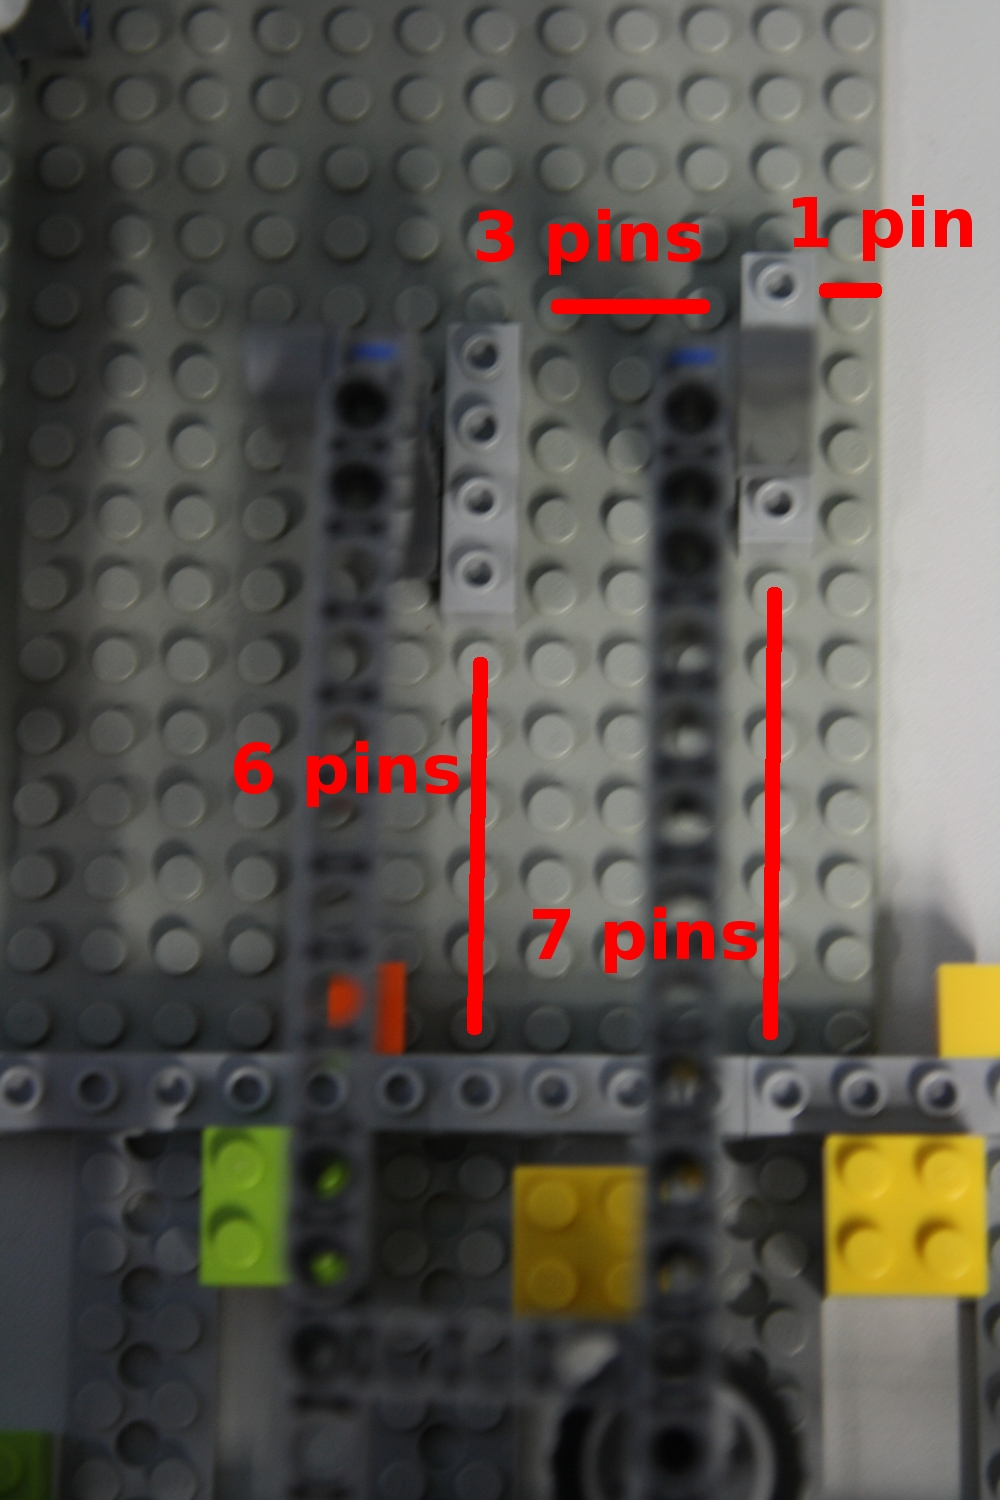
\includegraphics[scale=0.35]{graphics_lego/bridge2.jpg}
\end{center}
\caption{Position of the bridge}
\label{pic:bridge2}
\end{figure}

\newpage

Figure \ref{pic:bridge1} shows how the lower piers of the supporting bridge have to be placed in relation to the upper and right edge of the lower plate.

\begin{figure}[!htb]
\begin{center}
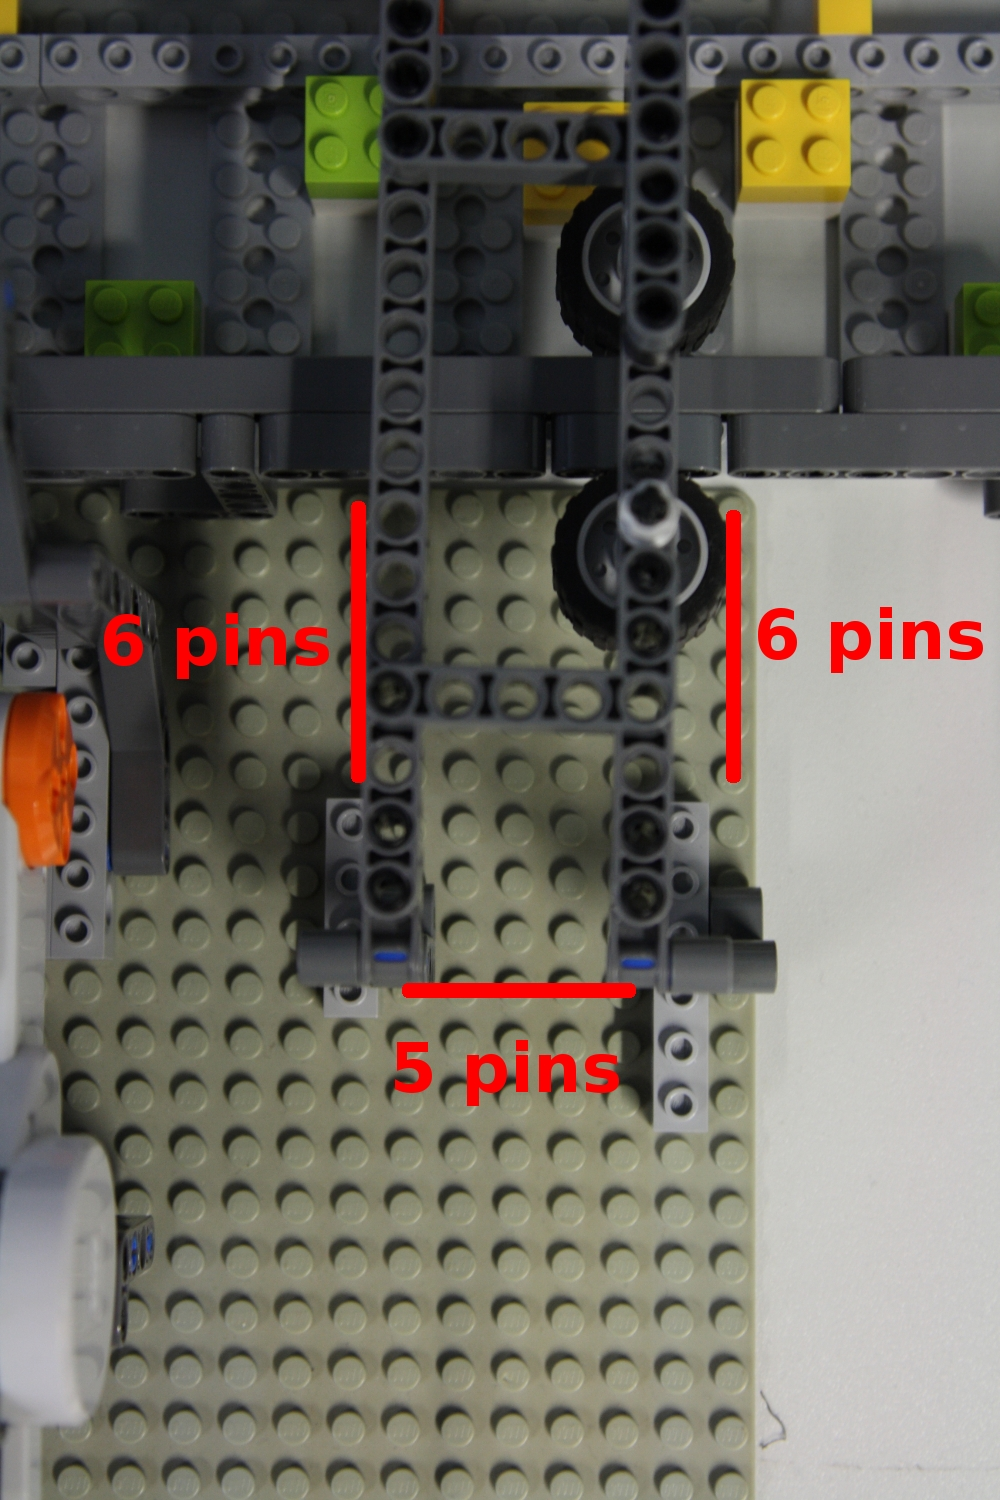
\includegraphics[scale=0.35]{graphics_lego/bridge1.jpg}
\end{center}
\caption{Position of the bridge}
\label{pic:bridge1}
\end{figure}

\newpage

\subsection{The sensors}

Figure \ref{pic:sensors} shows how the sensors have to be placed to work properly. As you can see the sensor it the rectangle 1 has to be above one of the position bits every time the sensors in rectangle 2 are above two bits at one of the positions.

\begin{figure}[!htb]
\begin{center}
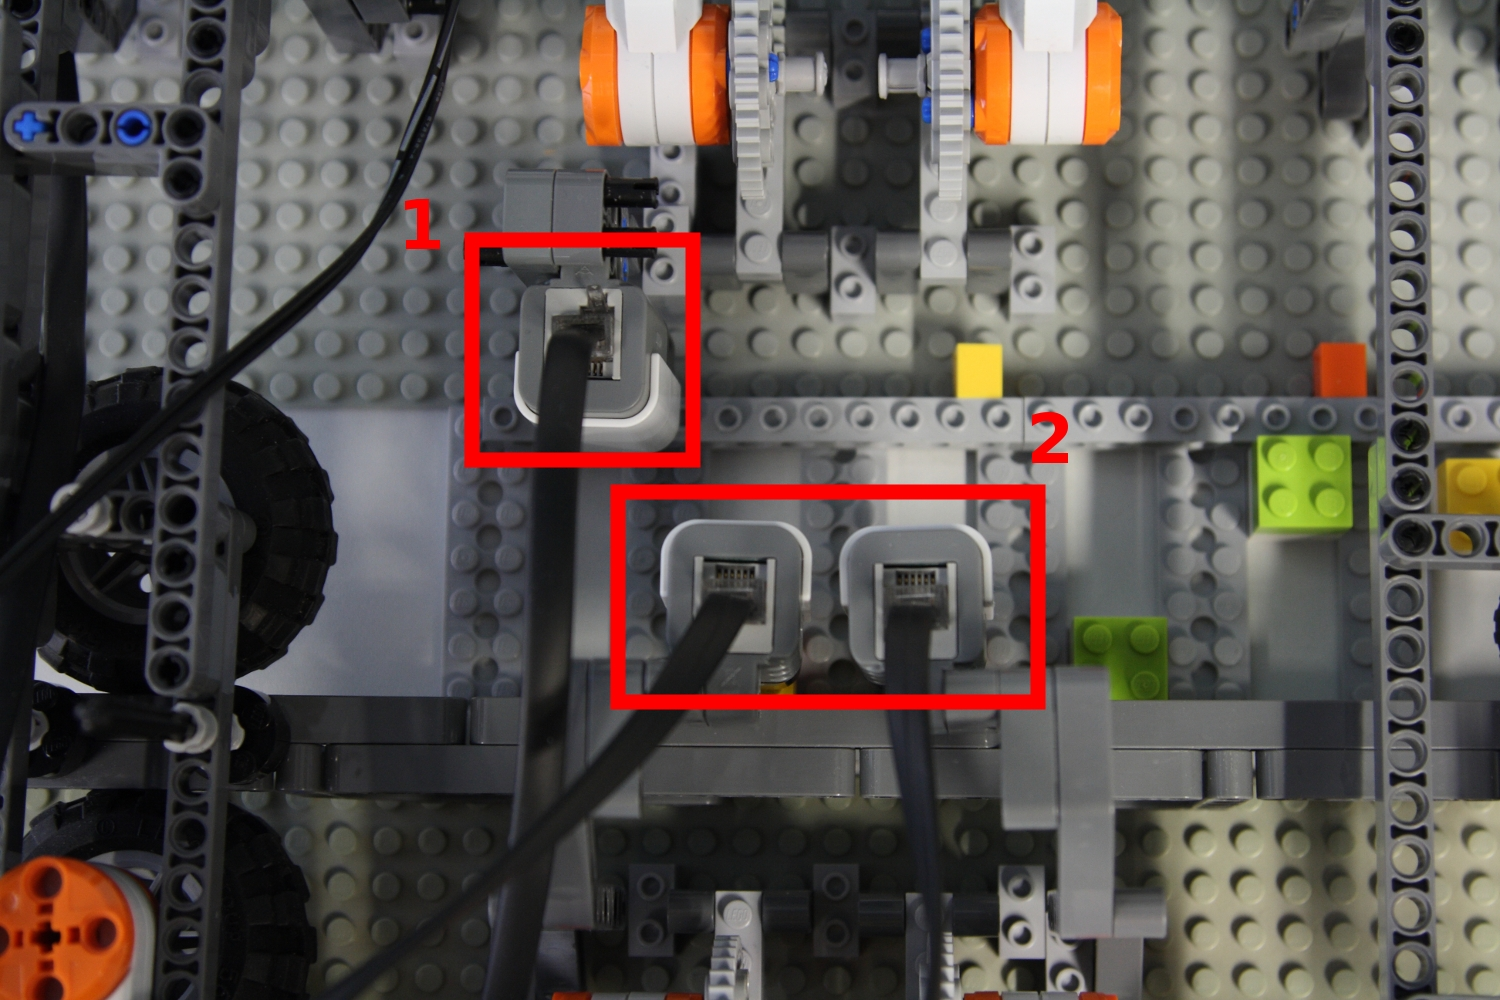
\includegraphics[scale=0.3]{graphics_lego/sensors.jpg}
\end{center}
\caption{Position of the sensors}
\label{pic:sensors}
\end{figure}

\newpage

\subsection{The tape}

The Marker in Figure \ref{pic:tape} shows how the bricks have to be placed so the sensors recognize them and can distinguish the different positions of the tape. It is also very important that the piers used for the upper bar of the tape are not interfering with the pushers shown in Figure \ref{pic:topview_pushers} and Figure \ref{pic:pusher}. So the pier you can see in the background of Figure \ref{pic:tape} is placed perfectly because it is not preventing the pushers from moving the bits.

\begin{figure}[!htb]
\begin{center}
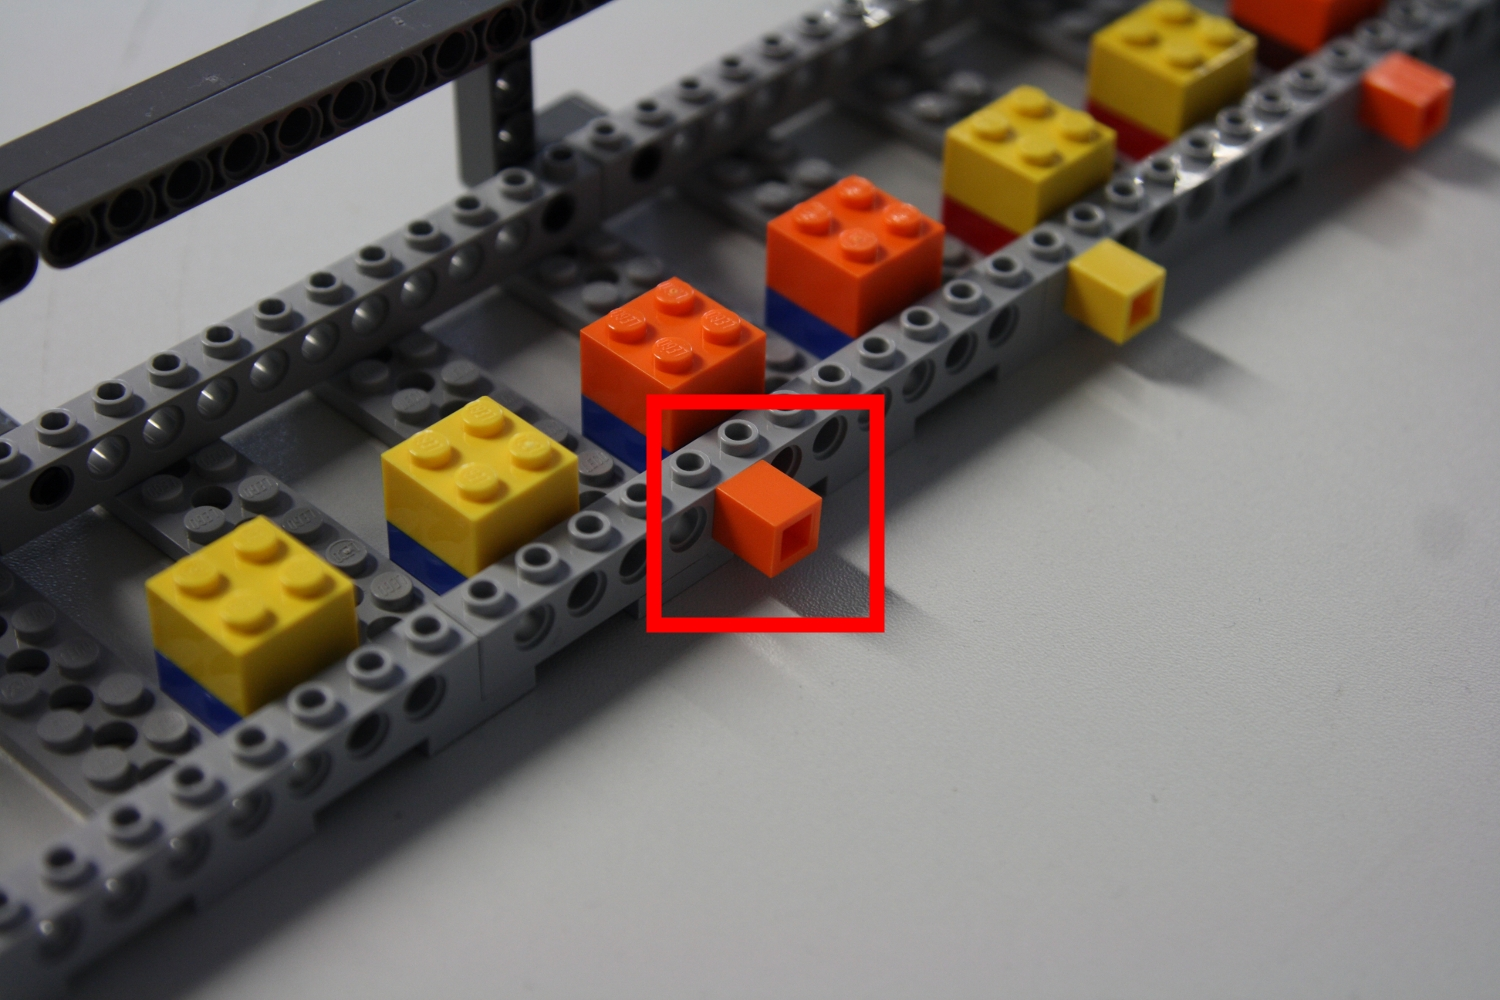
\includegraphics[scale=0.3]{graphics_lego/tape.jpg}
\end{center}
\caption{The tape}
\label{pic:tape}
\end{figure}

\newpage

Figure \ref{pic:supporting_pier} shows how the supporting piers have to be placed so they do not interfere with the pushers. It also shows how the sensors in the rectangle 2 in figure \ref{pic:sensors} have to be placed so they are above the bits every time the sensor in rectangle 1 is above a position bit.

\begin{figure}[!htb]
\begin{center}
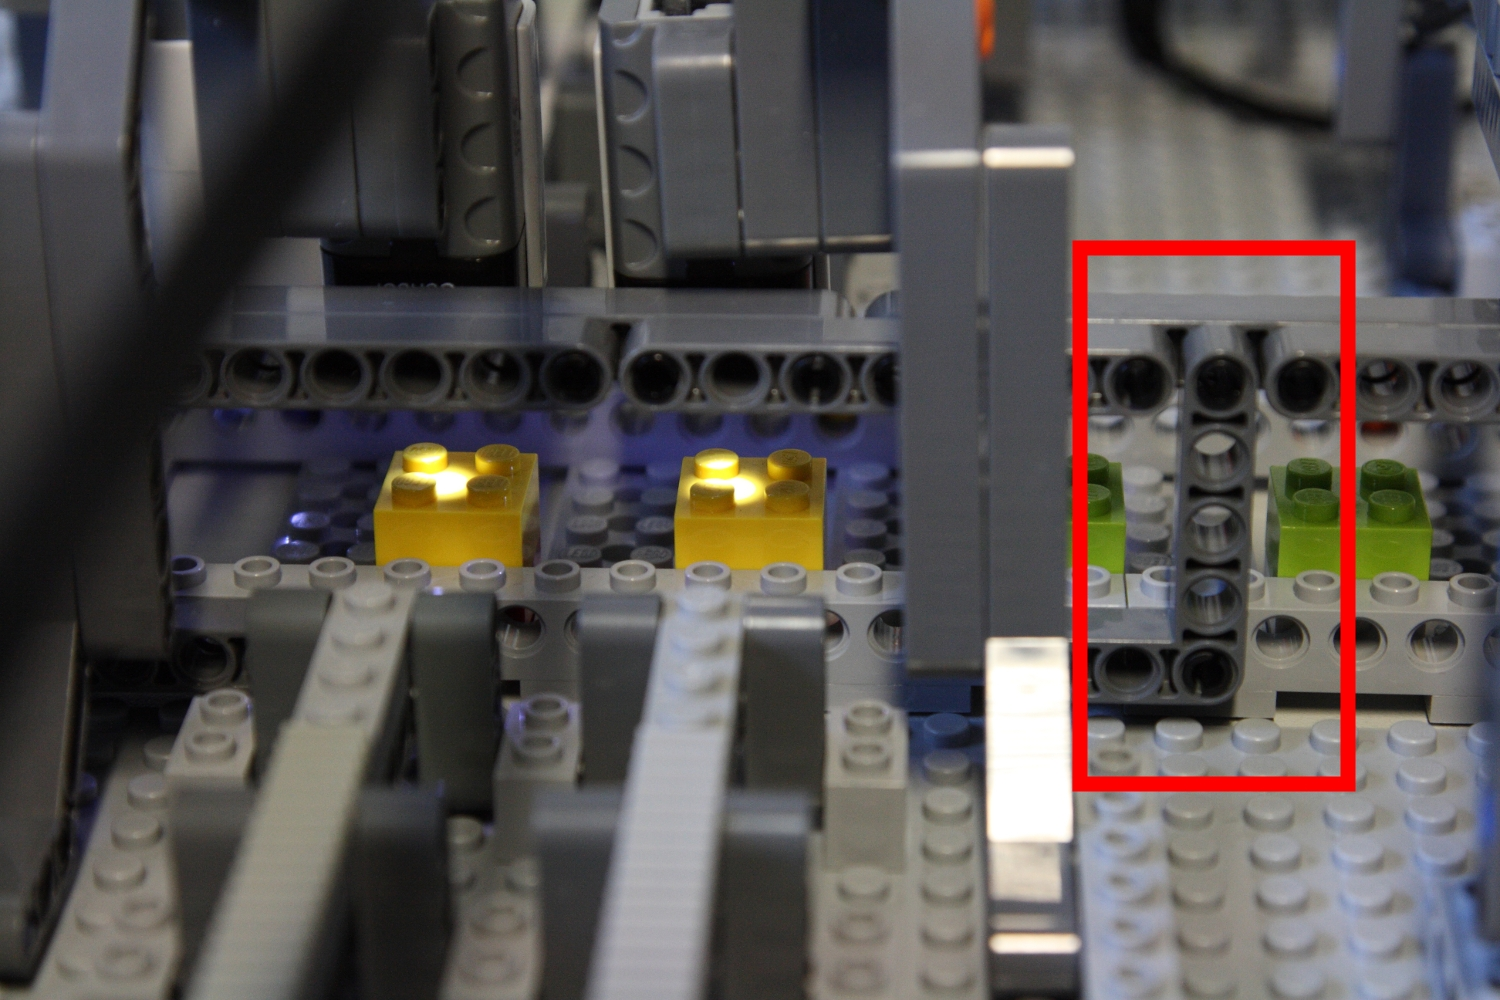
\includegraphics[scale=0.3]{graphics_lego/supporting_pier.jpg}
\end{center}
\caption{One of the supporting piers}
\label{pic:supporting_pier}
\end{figure}

\newpage

\subsection{The pushers}

Figure \ref{pic:pusher} shows how the pushers have to be placed on the guard rail so they can be pushed properly by the gear wheels. It also shows how the gear wheel has to be placed on the pusher so it pushes properly.

\begin{figure}[!htb]
\begin{center}
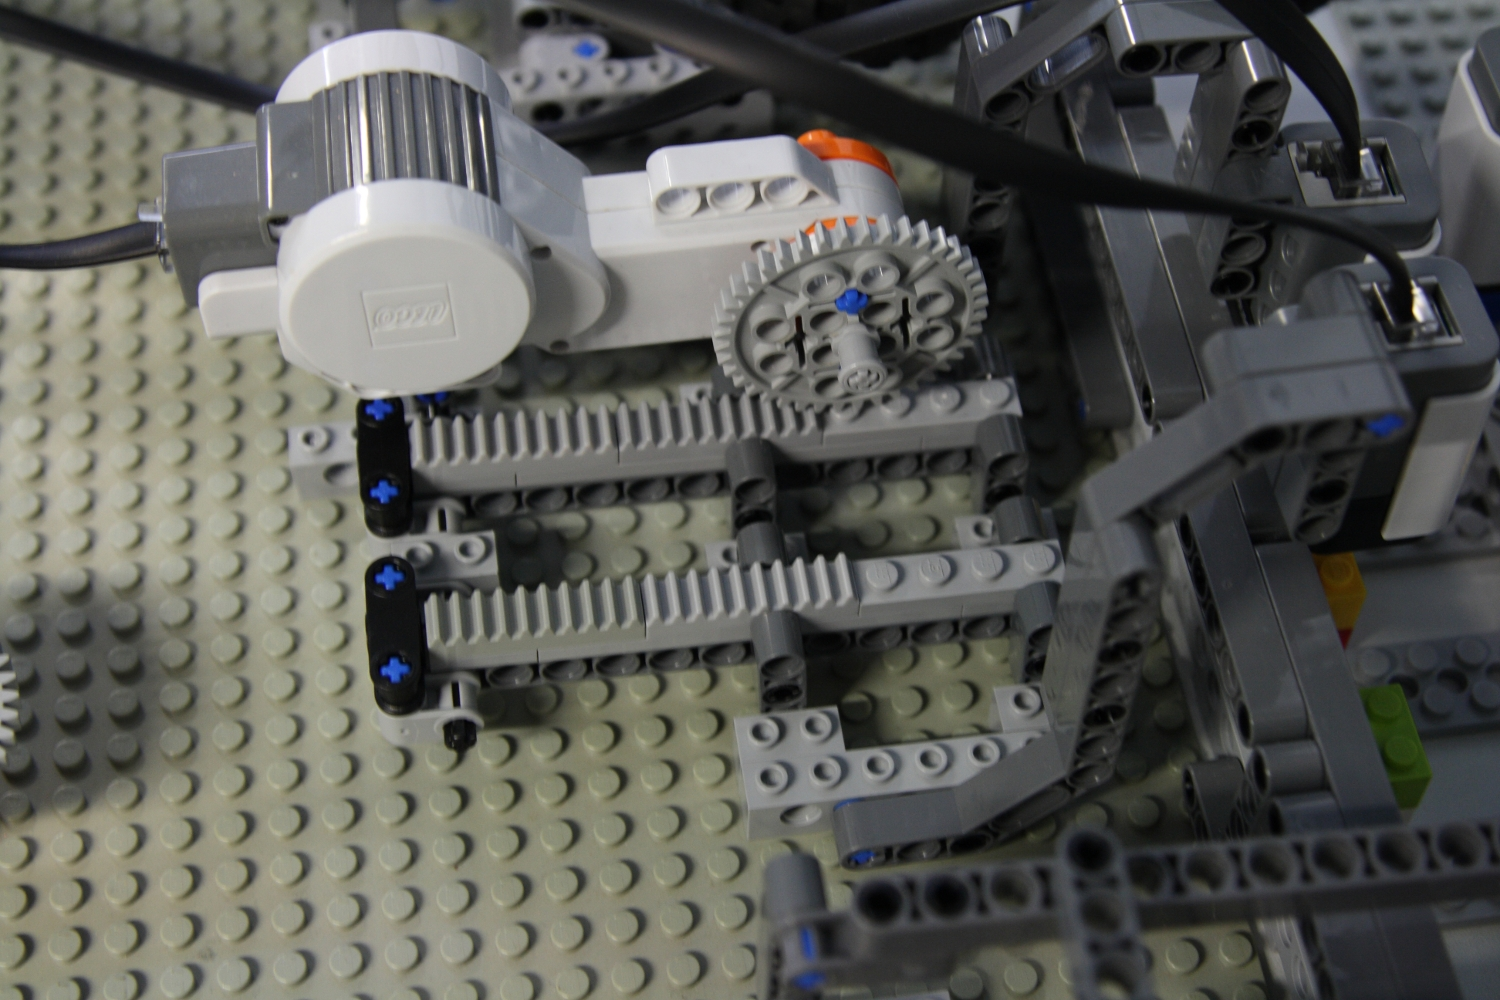
\includegraphics[scale=0.3]{graphics_lego/pusher.jpg}
\end{center}
\caption{Pusher}
\label{pic:pusher}
\end{figure}

\newpage

Figure \ref{pic:topview_pushers} shows how the pushers are pushing the bits and how to place the supporting piers (rectangle) for the tape's upper bar so they do not interfere with the pushers.

\begin{figure}[!htb]
\begin{center}
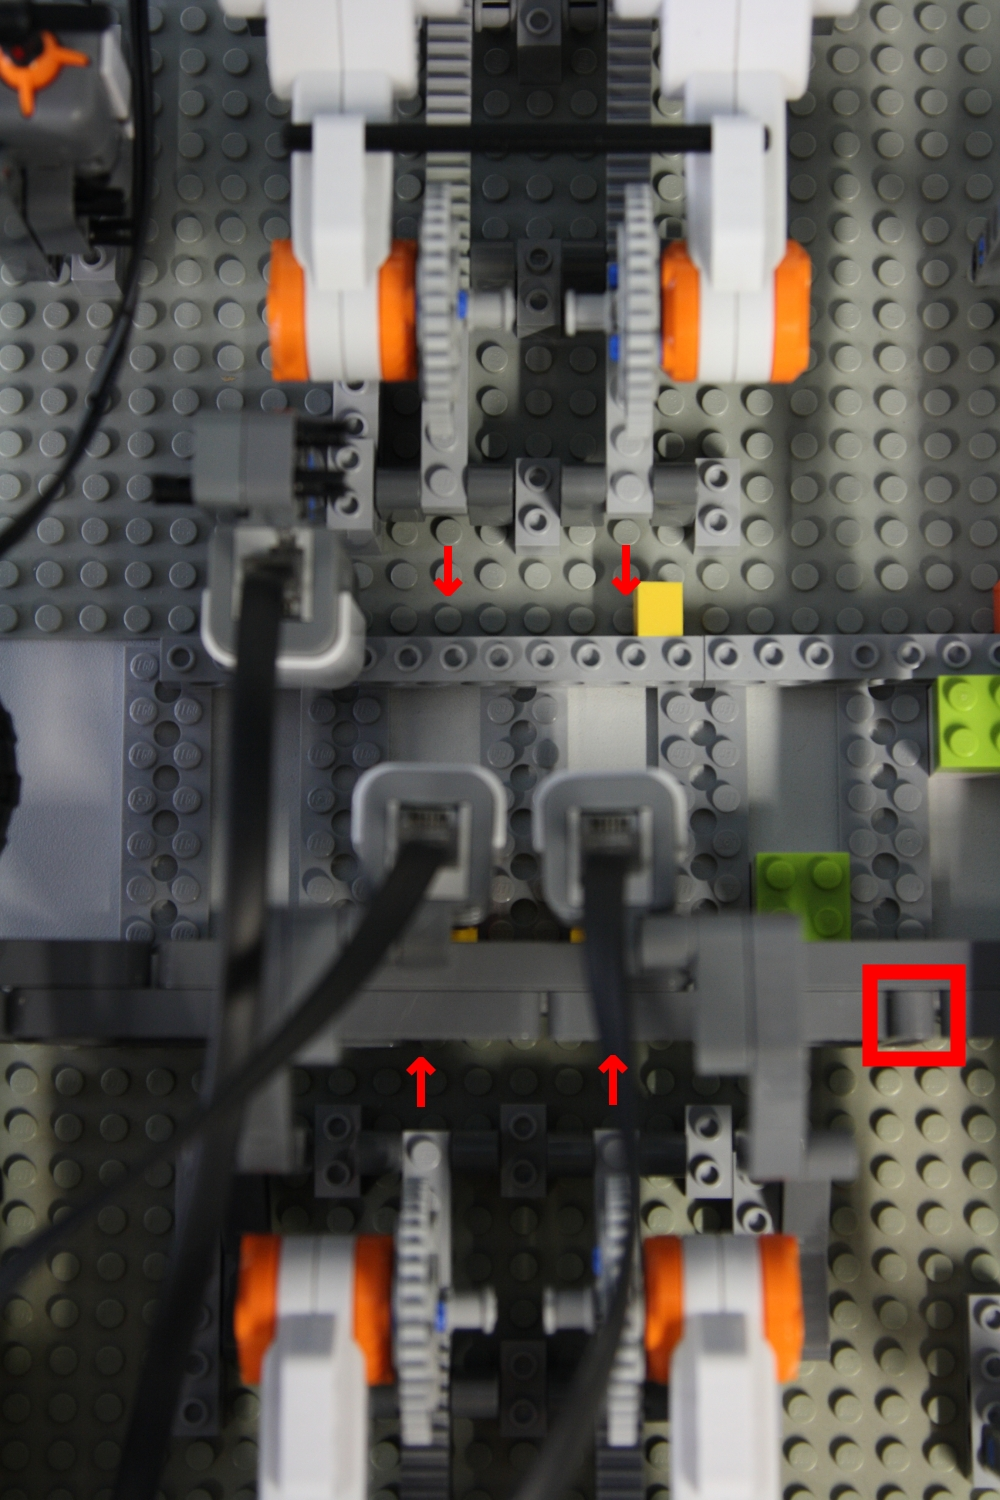
\includegraphics[scale=0.35]{graphics_lego/topview_pushers.jpg}
\end{center}
\caption{Position of the pushers}
\label{pic:topview_pushers}
\end{figure}


\makebackpage[trisec]%[<plain/info/addressinfo>]

\end{document}
